\begin{figure}[htbp]
  \centering
  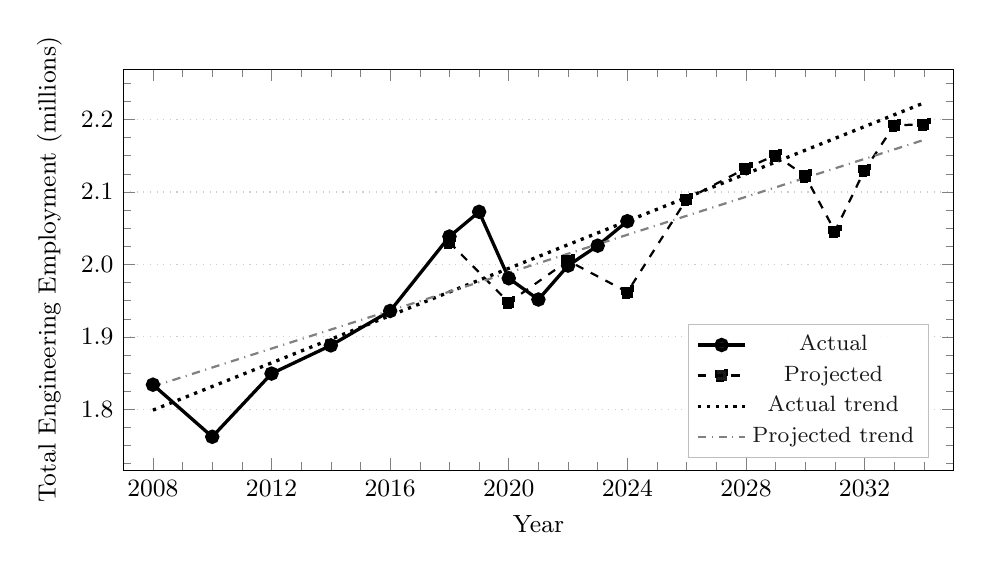
\begin{tikzpicture}
    \begin{axis}[
      width=\linewidth,
      height=0.55\linewidth,
      xlabel={Year},
      ylabel={Total Engineering Employment (millions)},
      xmin=2007, xmax=2035,
      xtick distance=4,
      minor tick num=3,
      x tick label style={/pgf/number format/1000 sep={}},
      y filter/.code={\pgfmathparse{#1/1000}\pgfmathresult},
      yticklabel={\pgfmathprintnumber[fixed,precision=1,zerofill]{\tick}},
      ymajorgrids=true,
      grid style={dotted,gray!40},
      legend pos=south east,
      legend style={font=\footnotesize, draw=gray!50, fill=white, fill opacity=0.9},
      tick label style={font=\small},
      label style={font=\small},
    ]
    % --- Actual employment ---
    \addplot[
      black, solid, very thick,
      mark=*, mark size=2pt,
    ] coordinates {(2008,1834.1) (2010,1762.2) (2012,1849.4) (2014,1888.3) (2016,1935.8) (2018,2038.5) (2019,2072.6) (2020,1980.9) (2021,1951.6) (2022,1998.4) (2023,2025.9) (2024,2059.7)};
    \addlegendentry{Actual}
    % --- Projected employment (one point per BLS edition) ---
    \addplot[
      black, dashed, thick,
      mark=square*, mark size=2pt,
    ] coordinates {(2018,2030.5) (2020,1947.5) (2022,2005.1) (2024,1961.9) (2026,2090.1) (2028,2132.7) (2029,2150.8) (2030,2122.0) (2031,2045.8) (2032,2130.1) (2033,2191.8) (2034,2193.5)};
    \addlegendentry{Projected}
    % --- Linear regression: actuals ---
    \addplot[
      black, dotted, very thick,
    ] coordinates {(2008,1799.0) (2034,2222.8)};
    \addlegendentry{Actual trend}
    % --- Linear regression: projections ---
    \addplot[
      gray, dashdotted, thick,
    ] coordinates {(2008,1831.6) (2034,2171.8)};
    \addlegendentry{Projected trend}
    \end{axis}
  \end{tikzpicture}
  \captiondatasource{US Engineering Employment, Actual and Projected}{\cite{u.s.bureauoflaborstatisticsOccupationalProjectionsWorker2024}}
  \label{fig:litReview-employmentTrend}
\end{figure}
